\chapter{Array Evaluation}
\section{Overview}
As stated in chapter \dots the geometry of a microphone array
has a impact on the performance of beamforming.
The goal is to find a well suited array geometry for the detection and tracking of
Drones.
To achieve this, first some array geometries have been simulated and then
a prototype was built to gather information on how they perform in reality.
Then the real data were compared to the simulated data to
confirm the validity of the simulation.
In the next step the findings of the prototypes and simulations
were used to come up with a final array design.

\newpage
\section{Mechanical Design}
Mechanical drawings of testarrays

\subsection{Multi-Circular Array}
\begin{minipage}{\linewidth}
	\begin{wrapfigure}{r}{7.5cm}
		\vspace{-0.8cm}
		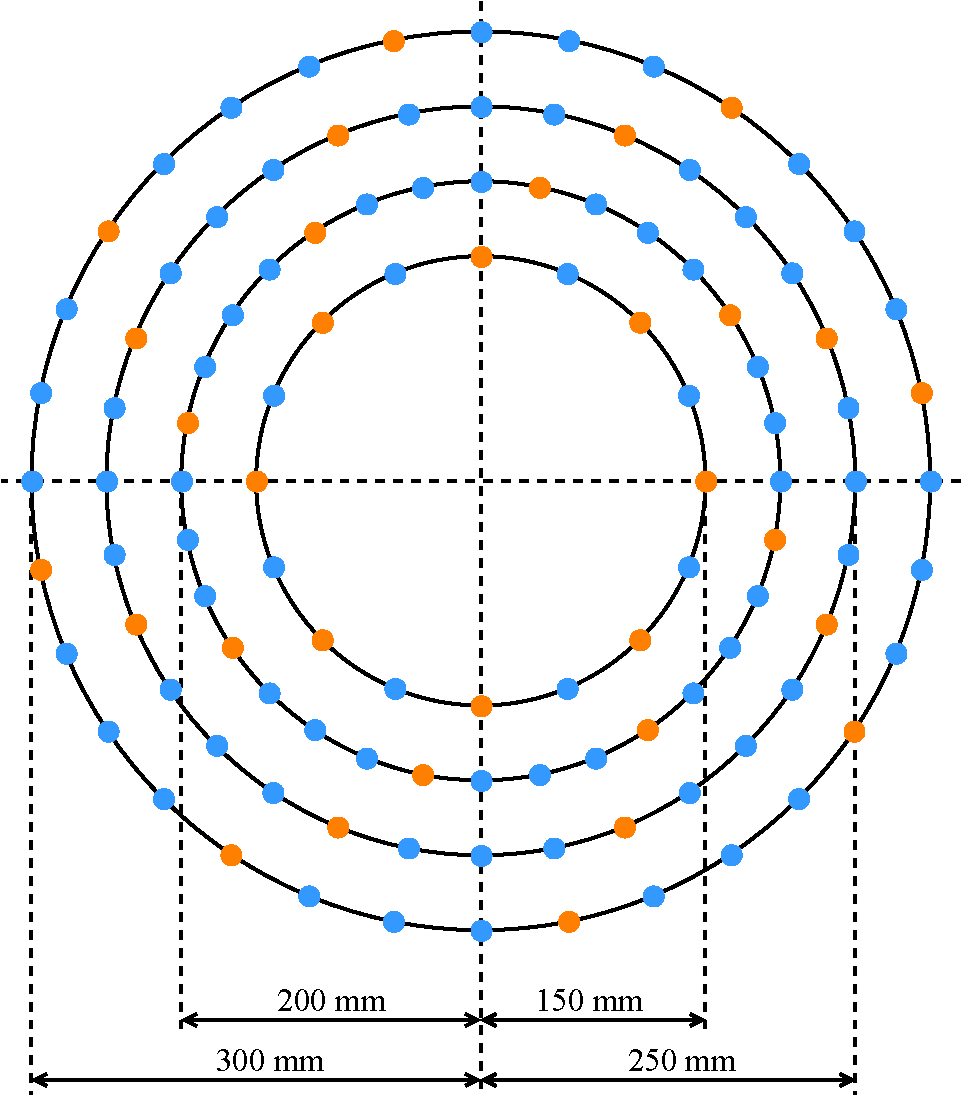
\includegraphics[width=7cm]{images/5_array_evaluation/prototype_array_multi_circular.pdf}
		\centering
		\caption{Multi-Circular Array}
		\label{fig:prototype_array_multi_circular}
	\end{wrapfigure}
	Lorem ipsum dolor sit amet, consetetur sadipscing elitr, sed diam nonumy eirmod tempor invidunt ut labore et dolore magna aliquyam erat, sed diam voluptua.
	At vero eos et accusam et justo duo dolores et ea rebum. Stet clita kasd gubergren, no sea takimata sanctus est Lorem ipsum dolor sit amet.
	Lorem ipsum dolor sit amet, consetetur sadipscing elitr, sed diam nonumy eirmod tempor invidunt ut labore et dolore magna aliquyam erat, sed diam voluptua.
	At vero eos et accusam et justo duo dolores et ea rebum
	\todo[inline]{\@Alain: Add explanation of the array geometry here}
\end{minipage}
\vspace{0.5cm}    % Adjust this depending on the length of the text above

\subsection{Archimedean Spiral Array}

\subsection{Wooden Prototype Arrays}

\begin{figure}[h!]
	\centering
	\begin{minipage}{0.49\textwidth}
		\centering
		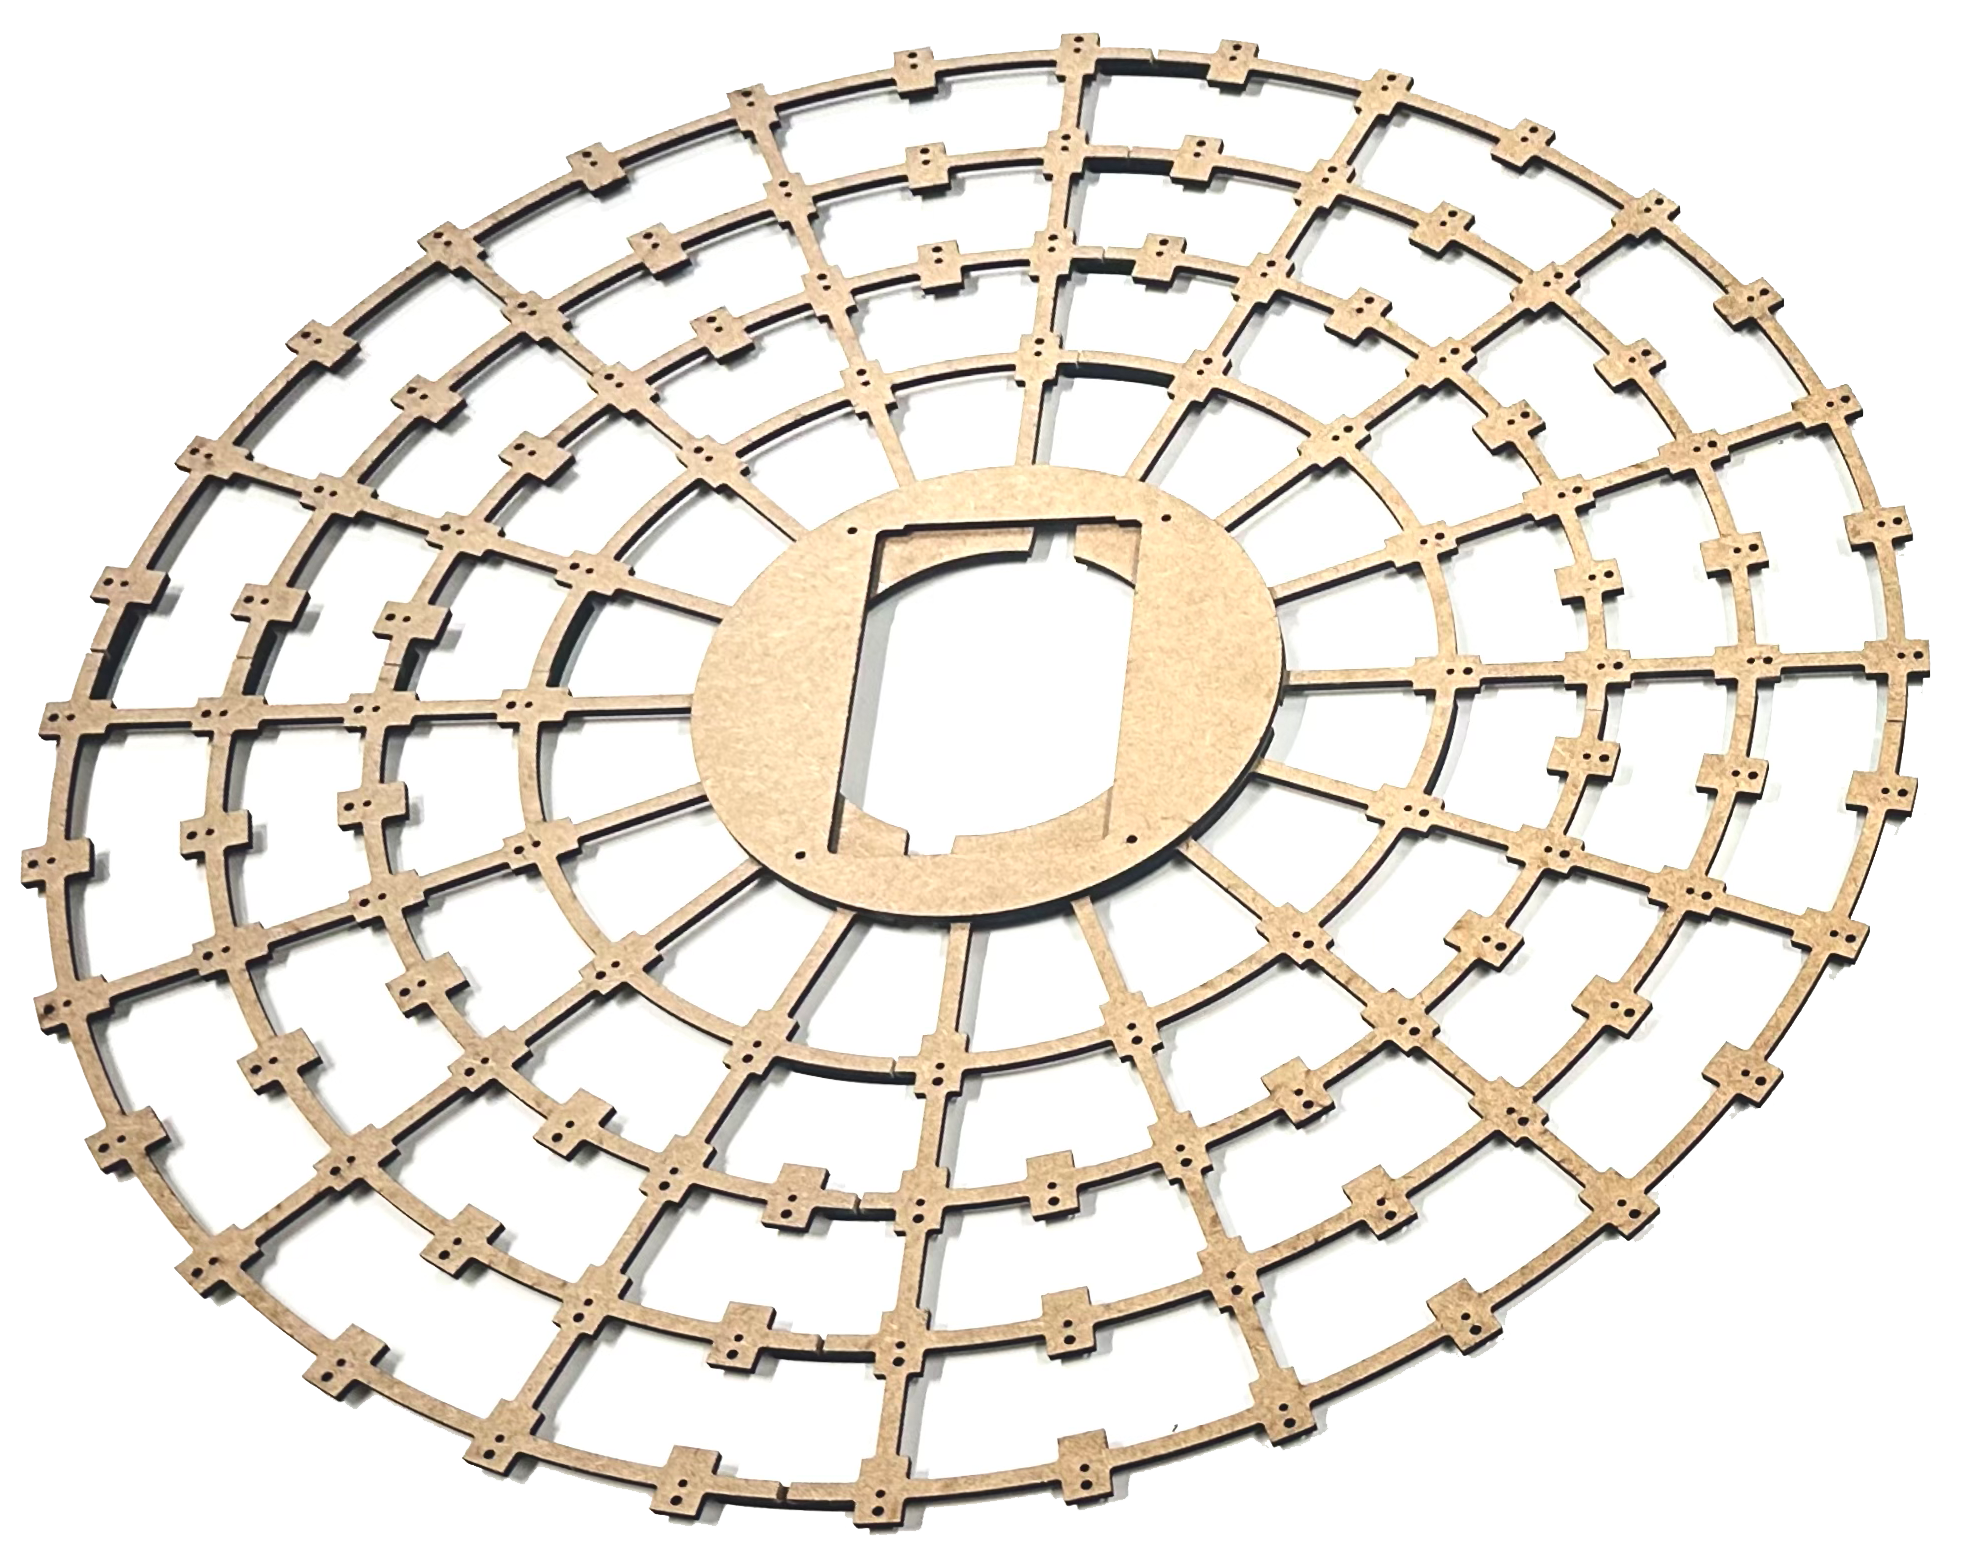
\includegraphics[width=0.95\textwidth]{images/5_array_evaluation/wooden_circular_array.png}
		\caption{Wooden Circular Array}
		\label{fig:wooden_circular_array}
	\end{minipage}
	\begin{minipage}{0.49\textwidth}
		\centering
		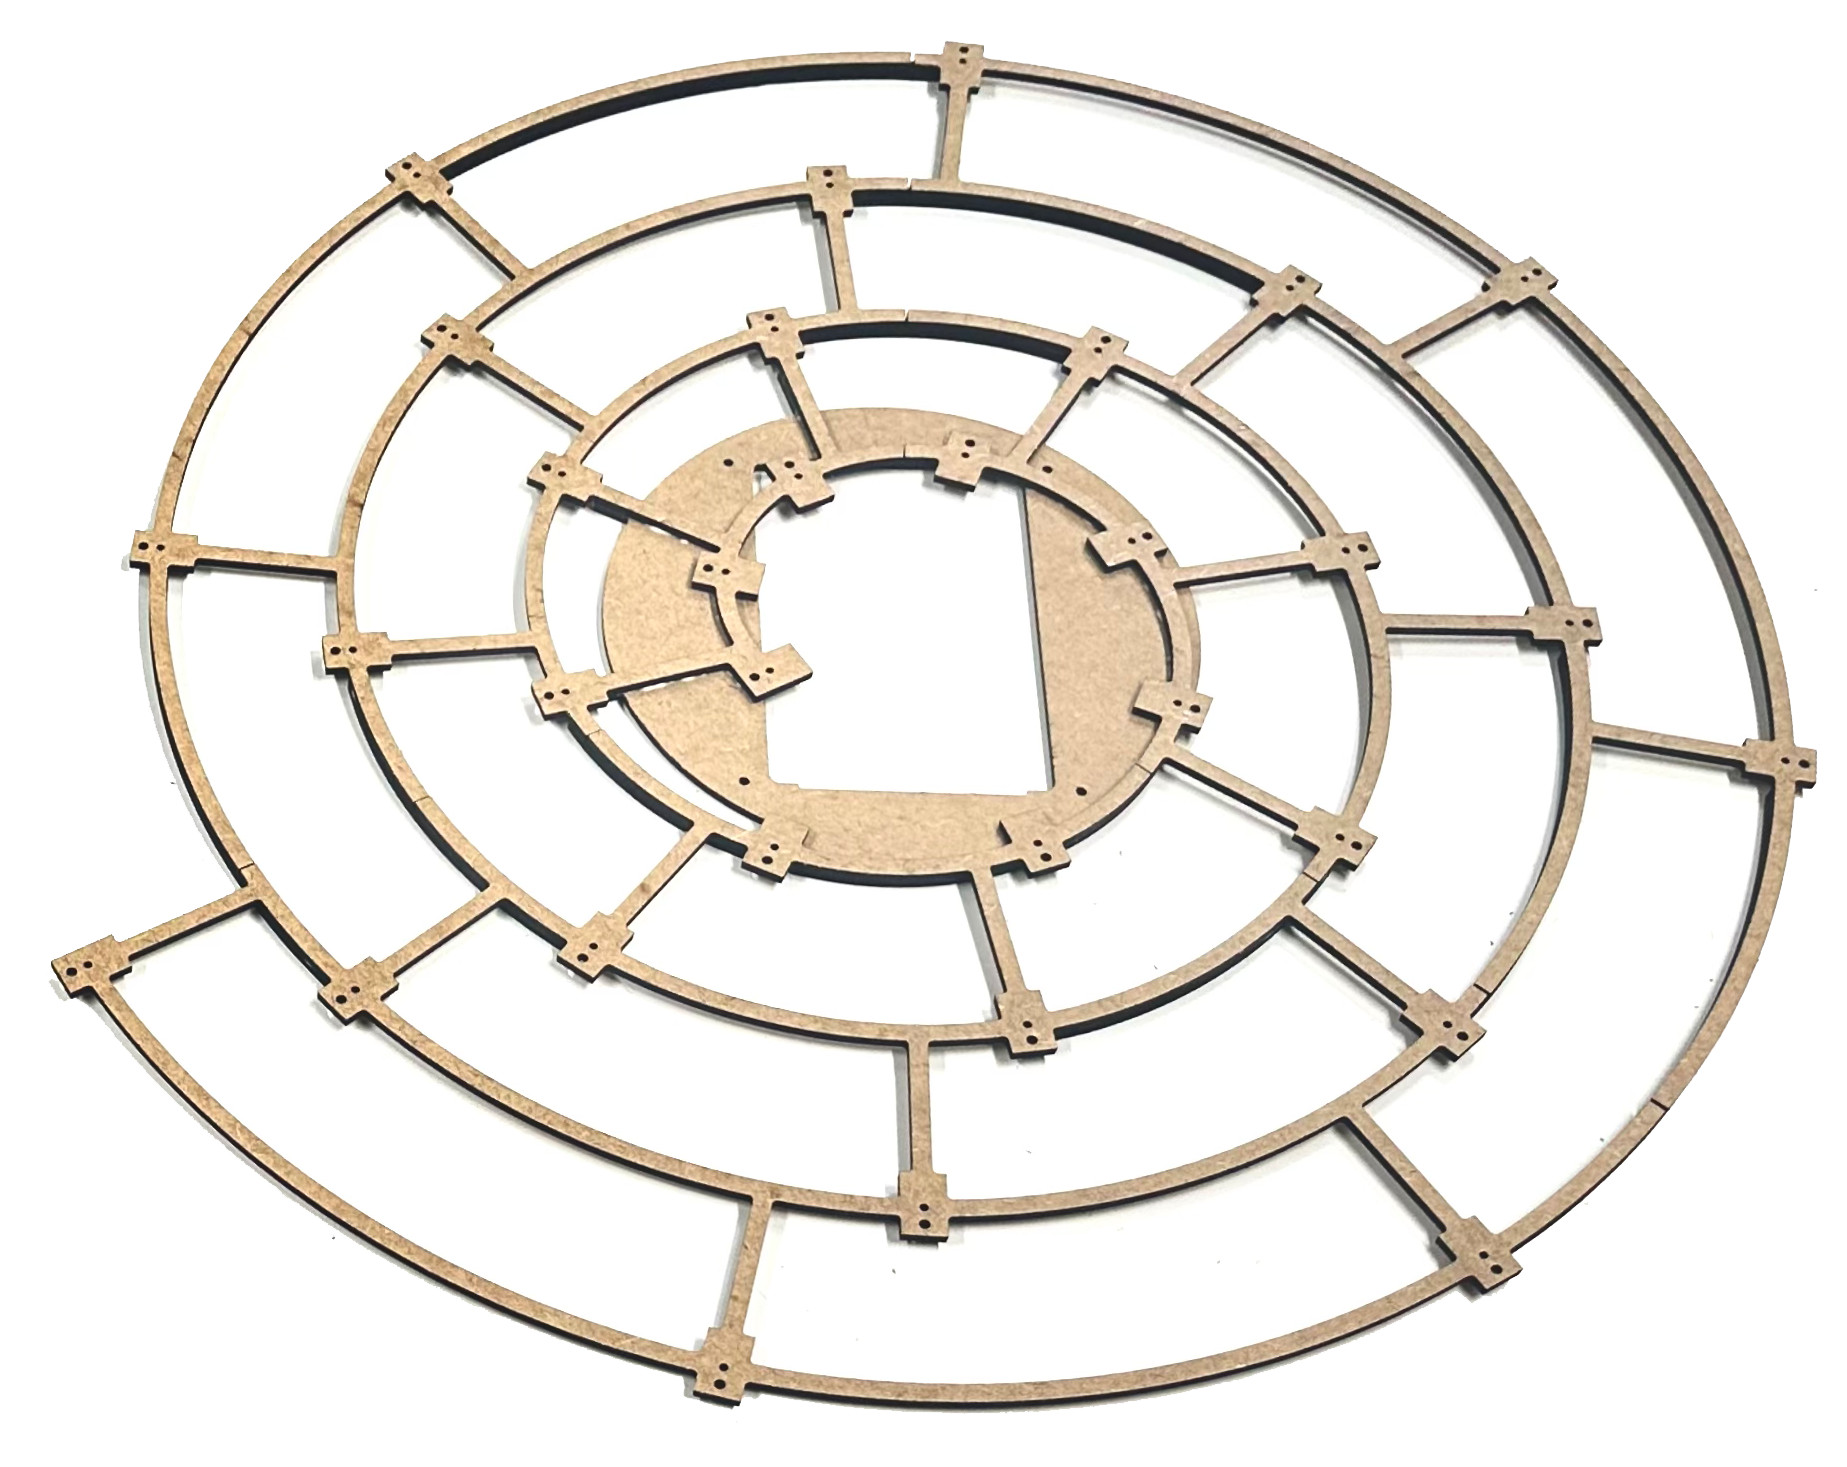
\includegraphics[width=0.95\textwidth]{images/5_array_evaluation/wooden_archimedean_spiral_array.png}
		\caption{Wooden Archimedean Spiral Array}
		\label{fig:wooden_archimedean_spiral_array}
	\end{minipage}
\end{figure}
\newpage


\section{Metrics}
TO evaluate the performance of an array several metrics are used.
In \todo{Cite Array design s40430-018-1275-5-1, array design comparisons} the
main beam-width is proposed.
\todo{cite Circ array drone trackings13638-019-1632-9} is using the ratio
between the main lobe power and the side lobe power.
Another measure related to the main lobe with is the main lobe area.
The main lobe is defined as all the points around the peak where their value
is greater than half the peaks value. \todo{besser englisch}

Blabla
\section{Array Geometry}
In \todo{cite} the authors use a circular array to detect and track drones.
They however did not gave any reasoning no why the chose a circular array.
\dots

\newpage
\section{Measurements \& Findings}
Blabla


\newpage
\section{Final Array Design}
Blabla
